
\section[Auswertung der Regleroptimierung am Motor mit Schwungmasse]{
    \parbox[t]{\dimexpr\textwidth\relax}{
Auswertung der Regleroptimierung am\\Motor mit Schwungmasse}}

\subsection{Synthetisierte Regler}

% tripple minipage
\begin{figure}[H]
    \centering
    \begin{minipage}[t]{0.32\textwidth}
        \begin{table}[H]
            \center
            \begin{tabular}{@{}cr@{}}
                    \toprule
                    \textbf{Parameter}              & \textbf{Wert} \\
                    \midrule
                    $Kp$                            & -0.411 \\[0.5ex]
                    $Ki$                            & -4.69e-8 \\[0.5ex]
                    $Kd$                            & -0.733 \\[0.5ex]
                    $Kn$                            & 12.453 \\[0.5ex]
                    \textbf{Konstante}              & \textbf{Wert} \\
                    $u_\mathbf{satHigh}$            & 10 \\[0.5ex]
                    $u_\mathbf{satLow}$             & -10 \\[0.5ex]
                    $I_{\mathbf{SatHigh}}$          & 100000000 \\[0.5ex]
                    $I_{\mathbf{SatLow}}$           & -100000000 \\[0.5ex]
                    Anti-Windup                     & Clamping \\[0.5ex]
                    \bottomrule
            \end{tabular}
            \caption{Reglerparameter des mit \textit{systune} optimierten Reglers}
            \label{tab:MotorMitSchwungmasseSystune_OptimizationParameters}
        \end{table}
    \end{minipage}
    \hfill
    \begin{minipage}[t]{0.32\textwidth}
        \begin{table}[H]
            \center
            \begin{tabular}{@{}cr@{}}
                    \toprule
                    \textbf{Parameter}              & \textbf{Wert} \\
                    \midrule
                    $Kp$                            & -0.771 \\[0.5ex]
                    $Ki$                            & -5.8e-5 \\[0.5ex]
                    $Kd$                            & -0.605 \\[0.5ex]
                    $Kn$                            & 4.065 \\[0.5ex]
                    \textbf{Konstante}              & \textbf{Wert} \\
                    $u_\mathbf{satHigh}$            & 10 \\[0.5ex]
                    $u_\mathbf{satLow}$             & -10 \\[0.5ex]
                    $I_{\mathbf{SatHigh}}$          & 100000000 \\[0.5ex]
                    $I_{\mathbf{SatLow}}$           & -100000000 \\[0.5ex]
                    Anti-Windup                     & Clamping \\[0.5ex]
                    \bottomrule
            \end{tabular}
            \caption{Reglerparameter des mit \gls{GA} optimierten Reglers}
            \label{tab:MotorMitSchwungmasseGA_OptimizationParameters}
        \end{table}
    \end{minipage}
    \hfill
    \begin{minipage}[t]{0.32\textwidth}
        \begin{table}[H]
            \center
            \begin{tabular}{@{}cr@{}}
                    \toprule
                    \textbf{Parameter}              & \textbf{Wert} \\
                    \midrule
                    $Kp$                            & -0.88 \\[0.5ex]
                    $Ki$                            & -9.48e-5 \\[0.5ex]
                    $Kd$                            & -0.635 \\[0.5ex]
                    $Kn$                            & 4.39 \\[0.5ex]
                    \textbf{Konstante}              & \textbf{Wert} \\
                    $u_\mathbf{satHigh}$            & 10 \\[0.5ex]
                    $u_\mathbf{satLow}$             & -10 \\[0.5ex]
                    $I_{\mathbf{SatHigh}}$          & 100000000 \\[0.5ex]
                    $I_{\mathbf{SatLow}}$           & -100000000 \\[0.5ex]
                    Anti-Windup                     & Clamping \\[0.5ex]
                    \bottomrule
            \end{tabular}
            \caption{Reglerparameter des mit \gls{DE} optimierten Reglers}
            \label{tab:MotorMitSchwungmasseDE_OptimizationParameters}
        \end{table}
    \end{minipage}
\end{figure}

\subsection{Systemverhalten am realen Prozess}
\begin{figure}[H]
	\center
    %\vspace{-1.6cm}
    \includegraphics[width=\linewidth]{images/MotorMitSchwungmasse/CombinedMethodes_realResult.pdf}
    \caption{Kombinierte Antwort auf Stimulation der optimierten Regler am Motor mit Schwungmasse}
    \label{fig:MotorMitSchwungmasseCombinedMethodes_realResult}
\end{figure}

\definecolor{systuneColor}{HTML}{3189f5}
\definecolor{geneticColor}{HTML}{2cf533}
\definecolor{differentialColor}{HTML}{cc2cf5}
\minipagedOrBelowEachOther
{
    In \ref{fig:MotorMitSchwungmasseCombinedMethodes_realResult} ist die Antwort auf die Stimulationssignale
    der drei Systeme dargestellt.
    Am realen System haben alle drei Regler mit den realen Bedingungen zu kämpfen.
    Die Reibungen im realen Prozess sorgen dafür,
    dass sich der Motor erst ab einem Wert von $\pm 400$ (normierter Wert: $\pm 1.33$) beginnt zu drehen und
    wenn das Motor Ansteuerungssignal auf $200$ (normierter Wert: $\pm 0.67$) absinkt bleibt der Motor stehen.
}
{
    Da diese Effekte im Modell nicht berücksichtigt wurden, haben die Optimierungsmethoden den I-Anteil des 
    Reglers nicht dementsprechend hoch genug gewählt, um diese Effekte zu kompensieren.
    Deshalb ist bei allen drei Reglern ein stationärer Fehler zu beobachten.
}

\minipagedOrBelowEachOther
{    
    \subparagraph{\textcolor{systuneColor}{\textit{Systune} Regler}}
        \noindent
        \\
        Der mit \textit{systune} optimierte Regler regelt das System deutlich langsamer als die beiden anderen Regler.

        
    \subparagraph{\textcolor{geneticColor}{Genetisch optimierter Regler}}
        \noindent
        \\
        Der mit \gls{GA} optimierte Regler zeigt 
        ein schnelleres Verhalten als der \textit{systune} Regler
}
{
	\subparagraph{\textcolor{differentialColor}{Differential Evolution optimierter Regler}}
        \noindent
        \\
        Der mit \gls{DE} optimierte Regler zeigt ein ziemlich ähnliches Verhalten wie 
        der mit \gls{GA} optimierte Regler. 
        Er verhält sich minimal besser als der \gls{GA} Regler.
}


\subsection{Lernverlauf}
\begin{figure}[H]
	\center
    %\vspace{-1.6cm}
    \includegraphics[width=\linewidth]{images/MotorMitSchwungmasse/CombinedMethodes_Simulation_LearningHistory_1.pdf}
    \caption{Lernverlauf der kombinierten Optimierungsmethoden (GA + DE)}
    \label{fig:MotorMitSchwungmasseCombinedMethodes_Simulation_LearningHistory_1}
\end{figure}

\minipagedOrBelowEachOther
{
    In~\ref{fig:MotorMitSchwungmasseCombinedMethodes_Simulation_LearningHistory_1} ist der Lernverlauf
    der beide Methoden \gls{GA} und \gls{DE} übereinandergelegt dargestellt. 
    Die Anzahl der Lernepochen ist auf 1000 gesetzt im Vergleich zum Beispiel mit dem DC-Motor mit 5000 Epochen.
    Der Grund liegt darin, dass die Frequenzanalyse sehr viel Rechenzeit beansprucht und die Durchläufe deshalb
    sehr lange dauern können ohne sehr viel Mehrwert zu bieten.

    
}
{
    Weil der GA zu Beginn der Optimierung die Verstärkungs- und Phasenreserve noch nicht 
    richtig berechnen kann, wird diese Bewertung erst ab Epoche 100 berücksichtigt. 
    Dadurch entsteht der Sprung im Lernverlauf des GA.
    Warum der DE diesen Sprung nicht hat, ist auf Seite
    \pageref{par:objektivesFazitDynamischeAnpassungBewertungsfunktion}: '\textbf{Dynamisches anpassen der Bewertungsfunktion}' erklärt.

    }

\horizontalLine
\minipagedOrBelowEachOther
{
    Der Lernverlauf ist leider für den \textit{systune} Regler nicht verfügbar, 
    damit dennoch ein Vergleich möglich ist wendet man die vom \textit{systune} berechneten Reglerparameter in der
    Simulationssoftware an und misst den Fehler mit der gleichen Bewertungsfunktion wie bei den anderen beiden Methoden.
    \textit{Systune} erreicht mit den in~\ref{tab:MotorMitSchwungmasseSystune_OptimizationParameters} angegebenen Parametern
    einen Fehler von $252.651$.
    % Params:
    % double Kp = -0.411;
    % double Ki = -4.69e-8;
    % double Kd = -0.733;
    % double Kn = 1/0.0803;
    % Integral Saturation High = 100000000.0;
    % Integral Saturation Low = -100000000.0;
    % Output Saturation High = 10;
    % Output Saturation Low = -10;
    %
    % Scores:
    % Score Component:  158.768  % absolut error
    % Score Component:  66.4595  % pid effort change
    % Score Component:  0        % overshoot
    % Score Component:  0        % Gain margin (not used)
    % Score Component:  27.8462  % Phase margin
    % Custom PID Test Score:  252.651    
}
{
    \textit{Systune} hat mit $252.651$ einen Fehler erreicht, der grösser als die Fehler von \gls{DE}
    und grösstenteils kleiner oder gleich den Fehlern von GA ist.
    Auch bei diesem System haben unterschiedliche Optimierungsziele einen wesentlichen Einfluss auf den erzielten Fehler von \textit{systune}.
    Der Vergleich des erreichten Fehlers mit dem GA optimierten Regler ist aufgrund des starken Sprunges im Lernverlauf sowieso schwierig.    
}



\newpage
\subsection{Frequenzanalyse der optimierten Regler}
%=== systunePID Performance ===
%Rise Time:        0.660 s
%Settling Time:    1.180 s
%Overshoot:        0.31 %
%
%Gain Margin:    19.83 dB
%Phase Margin:     75.71 °
%
%=== geneticPID Performance ===
%Rise Time:        0.498 s
%Settling Time:    2.222 s
%Overshoot:        24.03 %
%
%Gain Margin:    21.92 dB
%Phase Margin:     47.30 °
%
%=== differentialPID Performance ===
%Rise Time:        0.462 s
%Settling Time:    2.107 s
%Overshoot:        25.48 %
%
%Gain Margin:    21.25 dB
%Phase Margin:     46.30 °


%\horizontalLine
\minipagedOrBelowEachOther
{
    \vspace{0.6cm}
    Im \ref{fig:MotorMitSchwungmasseCombinedMethodes_PIDBode} sind die Bode-Diagramme der drei optimierten Regler dargestellt.
    Diese Zeigen die Frequenzgänge der Regler ohne die Regelstrecke.
    Der mit \textit{systune} optimierte Regler unterscheidet sich deutlich von den beiden anderen Reglern.
    \textit{Systune} hat für tiefe Frequenzen eine starke Dämpfung realisiert und eine konstante Verstärkung von ca. 20dB für hohe Frequenzen.

    Der \textit{systune} Regler wird also Rauschen am Eingang mit einer Verstärkung von Faktor 10 am Ausgang weitergeben.
    Die beiden anderen Regler zeigen ebenfalls eine Rauschverstärkung, jedoch mit einem Faktor von ca. 3.2 deutlich geringer.
    Der Regler vom \gls{GA} zeigt die kleinste Rauschverstärkung unter den drei Reglern. 
}
{
    \begin{figure}[H]
        \center
        %\vspace{-1.6cm}
        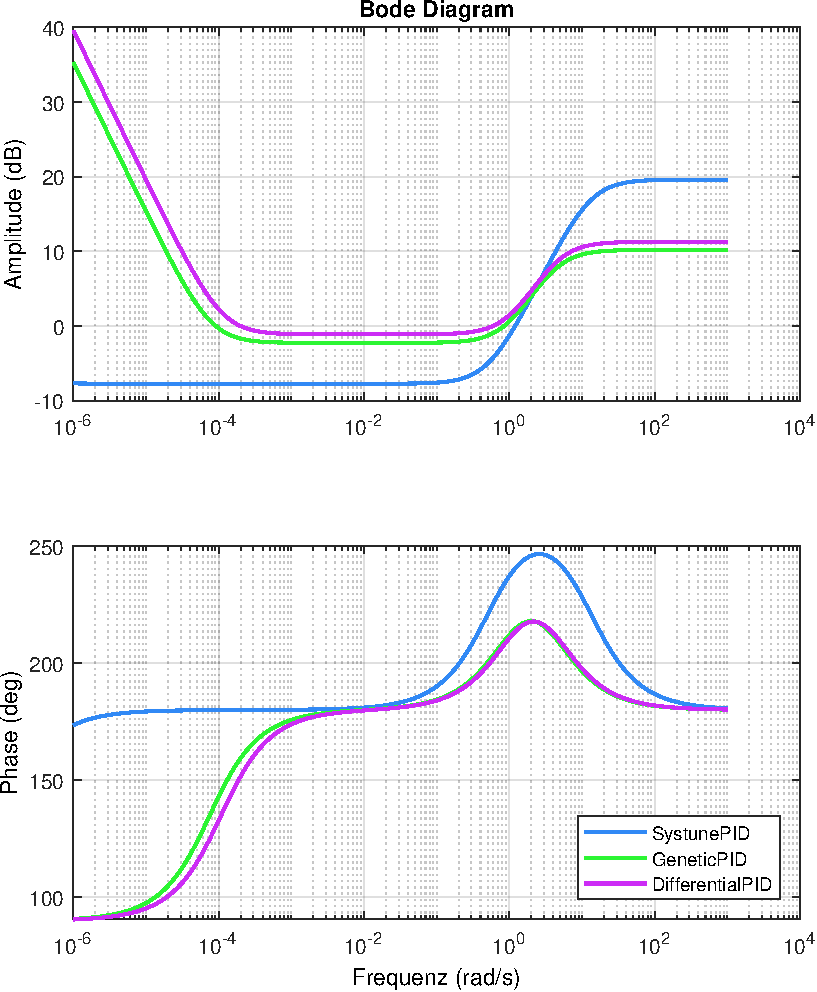
\includegraphics[width=\linewidth]{images/MotorMitSchwungmasse/CombinedMethodes_PIDBode.pdf}
        \caption{Bode-Diagramm der optimierten Regler}
        \label{fig:MotorMitSchwungmasseCombinedMethodes_PIDBode}
    \end{figure}
}

\newpage
\subsection{Frequenzanalyse der optimierten Systeme}
%\horizontalLine
\minipagedOrBelowEachOther
{
    \begin{figure}[H]
        \center
        %\vspace{-1.6cm}
        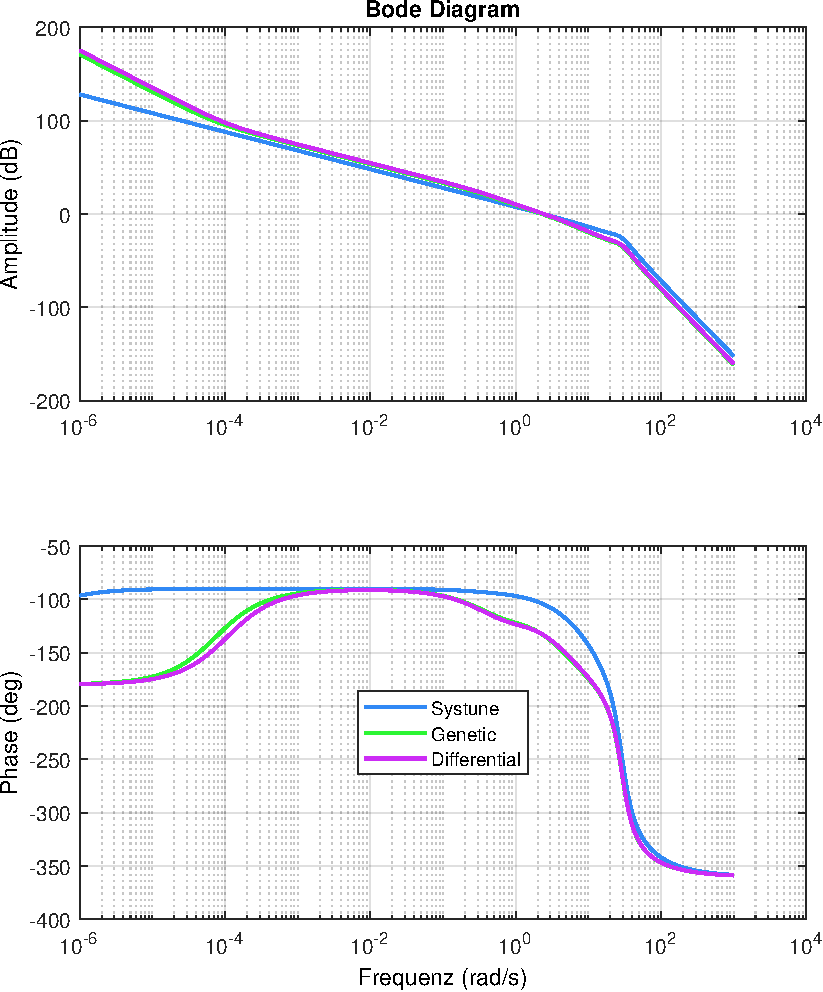
\includegraphics[width=\linewidth]{images/MotorMitSchwungmasse/CombinedMethodes_SystemBode.pdf}
        \caption{Bode-Diagramm der optimierten Vorwärts Pfade der einzelnen Systeme}
        \label{fig:MotorMitSchwungmasseCombinedMethodes_SystemBode}
    \end{figure}
    Das Bode-Diagramm in~\ref{fig:MotorMitSchwungmasseCombinedMethodes_SystemBode} und das
    Nyquist-Diagramm in~\ref{fig:MotorMitSchwungmasseCombinedMethodes_SystemLogScaleNyquist} zeigen,
    jeweils die Frequenzgänge der optimierten Vorwärts Pfade der drei Systeme:
    \begin{itemize}
        \item \textcolor{systuneColor}{$PID_{\mathbf{systune}} \cdot MotorSystem$}
        \item \textcolor{geneticColor}{$PID_{\mathbf{genetic}} \cdot MotorSystem$}
        \item \textcolor{differentialColor}{$PID_{\mathbf{differential}} \cdot MotorSystem$}
    \end{itemize}

    Im Nyquist-Diagramm fällt auf, dass der Regler von \textit{systune} seinem System deutlich mehr Phasenreserve bietet.
    Die Verstärkungsreserve ist bei den Reglern von GA und DE etwas höher als bei \textit{systune}, wobei aber 
    auch \textit{systune} mit 19.83dB eine sehr gute Verstärkungsreserve erreicht hat.  
}
{
    \begin{figure}[H]
        \center
        %\vspace{-1.6cm}
        \includegraphics[width=\linewidth]{images/MotorMitSchwungmasse/CombinedMethodes_SystemLogScaleNyquist.pdf}
        \vspace{-0.2cm}
        \caption{Logarithmisches Nyquist-Diagramm der optimierten Vorwärts Pfade der einzelnen Systeme \cite{matlabScriptNyquistLog}}
        \label{fig:MotorMitSchwungmasseCombinedMethodes_SystemLogScaleNyquist}
    \end{figure}

    \begin{table}[H]
        \center
        \begin{tabular}{@{}cr@{}}
                \toprule
                \textbf{Phasenreserve}              & \textbf{Wert} \\
                \midrule
                \textcolor{systuneColor}{\textit{Systune}}                          & 75.71 ° \\[0.5ex]
                \textcolor{geneticColor}{Genetisch}                        & 47.30 ° \\[0.5ex]
                \textcolor{differentialColor}{Differential Evolution}      & 46.30 ° \\[0.5ex]
                \hline
                \textbf{Verstärkungsreserve}              &  \\
                \hline
                \textcolor{systuneColor}{\textit{Systune}}                          & 19.83 dB \\[0.5ex]
                \textcolor{geneticColor}{Genetisch}                        & 21.92 dB \\[0.5ex]
                \textcolor{differentialColor}{Differential Evolution}      & 21.25 dB \\[0.5ex]
                \bottomrule
        \end{tabular}
        \caption{Reserven der optimierten Systeme}
        \label{tab:MotorMitSchwungmasseCombinedMethodes_AnalyzedData}
    \end{table}
}


\newpage
\subsection{Stabilitätsanalyse der optimierten Systeme}
\subsubsection{Sensitivität}
\begin{figure}[H]
    %\vspace{-1.6cm}
    \includegraphics[width=\linewidth]{images/MotorMitSchwungmasse/CombinedMethodes_Sensitivity.pdf}
    \caption{Sensitivität der optimierten Systeme}
    \label{fig:MotorMitSchwungmasseCombinedMethodes_Sensitivity}
\end{figure}
\minipagedOrBelowEachOther
{
    Das Sensitivitäts-Diagramm in \ref{fig:MotorMitSchwungmasseCombinedMethodes_Sensitivity} zeigt,
    für die mit \gls{GA} und \gls{DE} optimierten Systeme einen ähnlichen Verlauf.
    Beide haben eine stärkere Überhöhung im Vergleich zum mit \textit{systune} optimierten System.
    Insgesamt sind aber alle drei robuster gegenüber Totzeiten im Vergleich 
    zum System mit dem DC-Motor.
}
{

}

\horizontalLine
\begin{figure}[H]
    \subsubsection{Phasen- \& Verstärkungsreserve Diagramme der optimierten Systeme}
    \begin{minipage}[t]{0.32\textwidth}
        \begin{figure}[H]
            %\vspace{-1.6cm}
            \includegraphics[width=\linewidth]{images/MotorMitSchwungmasse/SystuneStabilityPhaseMarginsPlot.pdf}
            \caption{Phasen- \& Verstärkungsreserve des mit \textit{systune} optimierten Systems}
            \label{fig:MotorMitSchwungmasseSystuneStabilityPhaseMarginsPlot}
        \end{figure}
    \end{minipage}
    \hfill
    \begin{minipage}[t]{0.32\textwidth}
        \begin{figure}[H]
            %\vspace{-1.6cm}
            \includegraphics[width=\linewidth]{images/MotorMitSchwungmasse/GeneticStabilityPhaseMarginsPlot.pdf}
            \caption{Phasen- \& Verstärkungsreserve des mit Genetic optimierten Systems}
            \label{fig:MotorMitSchwungmasseGeneticStabilityPhaseMarginsPlot}
        \end{figure}
    \end{minipage}
    \hfill
    \begin{minipage}[t]{0.32\textwidth}
        \begin{figure}[H]
            %\vspace{-1.6cm}
            \includegraphics[width=\linewidth]{images/MotorMitSchwungmasse/DifferentialStabilityPhaseMarginsPlot.pdf}
            \caption{Phasen- \& Verstärkungsreserve des mit Differential Evolution optimierten Systems}
            \label{fig:MotorMitSchwungmasseDifferentialStabilityPhaseMarginsPlot}
        \end{figure}
    \end{minipage}


\minipagedOrBelowEachOther
{
    Die drei Diagramme in 
\ref{fig:MotorMitSchwungmasseSystuneStabilityPhaseMarginsPlot}, 
\ref{fig:MotorMitSchwungmasseGeneticStabilityPhaseMarginsPlot} und 
\ref{fig:MotorMitSchwungmasseDifferentialStabilityPhaseMarginsPlot}
    zeigen die detaillierten Stabilitätsreserven als Kombination von Verstärkung und 
    konstanter Phasenverschiebung.
    Wie diese Diagramme zu lesen sind, ist in folgendem Kapitel erklärt:\\
\fullref{sec:StabilitaetsPhaseMarginPlot}
}
{
    Die Stabile Region ist beim Regler von \textit{systune} am besten ausgeprägt. 
    Dieser bietet viel Spielraum für Phasenänderungen auch mit zusätzlicher Verstärkung.
    Die Regler von Genetic und Differential Evolution bieten eine ähnliche Stabile Region,
    welche nicht ganz so gross ist wie die von \textit{systune}.
}
\end{figure}


\newpage
\begin{figure}[H]
    \subsubsection{Totzeit- \& Verstärkungsreserve Diagramme der optimierten Systeme}
    \begin{minipage}[t]{0.32\textwidth}
        \begin{figure}[H]
            %\vspace{-1.6cm}
            \includegraphics[width=\linewidth]{images/MotorMitSchwungmasse/SystuneStabilityDelayMarginsPlot.pdf}
            \caption{Totzeit- \& Verstärkungsreserve des mit \textit{systune} optimierten Systems}
            \label{fig:MotorMitSchwungmasseSystuneStabilityDelayMarginsPlot}
        \end{figure}
    \end{minipage}
    \hfill
    \begin{minipage}[t]{0.32\textwidth}
        \begin{figure}[H]
            %\vspace{-1.6cm}
            \includegraphics[width=\linewidth]{images/MotorMitSchwungmasse/GeneticStabilityDelayMarginsPlot.pdf}
            \caption{Totzeit- \& Verstärkungsreserve des mit Genetic optimierten Systems}
            \label{fig:MotorMitSchwungmasseGeneticStabilityDelayMarginsPlot}
        \end{figure}
    \end{minipage}
    \hfill
    \begin{minipage}[t]{0.32\textwidth}
        \begin{figure}[H]
            %\vspace{-1.6cm}
            \includegraphics[width=\linewidth]{images/MotorMitSchwungmasse/DifferentialStabilityDelayMarginsPlot.pdf}
            \caption{Totzeit- \& Verstärkungsreserve des mit Differential Evolution optimierten Systems}
            \label{fig:MotorMitSchwungmasseDifferentialStabilityDelayMarginsPlot}
        \end{figure}
    \end{minipage}


\minipagedOrBelowEachOther
{
    Die drei Diagramme in 
\ref{fig:MotorMitSchwungmasseSystuneStabilityDelayMarginsPlot}, 
\ref{fig:MotorMitSchwungmasseGeneticStabilityDelayMarginsPlot} und 
\ref{fig:MotorMitSchwungmasseDifferentialStabilityDelayMarginsPlot}
    zeigen die detaillierten Stabilitätsreserven aus der Kombination von Verstärkung und 
    Totzeit.
    Wie diese Diagramme zu lesen sind, ist in folgendem Kapitel erklärt:\\
\fullref{sec:StabilitaetsDelayMarginPlot}
}
{
    Auch wenn die Verstärkungsreserve nicht beliebig gross ist, verhalten sich alle drei Systeme relativ robust
    gegenüber Kombinationen von Totzeit und Verstärkungsänderungen.
    Bei einer Verstärkung von 1, bleiben alle drei Systeme noch mit einer Totzeit von ca. 300ms stabil.
}
\end{figure}
\newpage